% chktex-file 2% chktex-file 29
% chktex-file 13
\documentclass{report}
\usepackage{setspace}
\usepackage[a4paper, total={7in, 10in}]{geometry}
\usepackage[fleqn]{amsmath}
\usepackage{empheq}
\usepackage{amssymb}
\usepackage{amsthm}
\usepackage{gensymb}
\usepackage[fleqn]{cases}
\usepackage{multicol}
\usepackage{color}
\usepackage{stix}
\usepackage{chngcntr}
\usepackage{tikz}
\usepackage{enumitem}
\usepackage{pgfplots}
\usepackage{etoolbox}
\usepackage{tikz-3dplot}
\usepackage{tkz-euclide}
\usepackage{graphicx}
\usepackage{enumitem}

\def\nswe#1#2#3{#1\,$#2^\circ\,#3'$}
\graphicspath{ {./assets/} }
\usetikzlibrary{calc,matrix,arrows}
\usetikzlibrary{decorations.pathmorphing,patterns, calligraphy, perspective,backgrounds}

\tikzset{
  right angle quadrant/.code={
      \pgfmathsetmacro\quadranta{{1,1,-1,-1}[#1-1]}     % Arrays for selecting quadrant
      \pgfmathsetmacro\quadrantb{{1,-1,-1,1}[#1-1]}},
  right angle quadrant=1, % Make sure it is set, even if not called explicitly
  right angle length/.code={\def\rightanglelength{#1}},   % Length of symbol
  right angle length=2ex, % Make sure it is set...
  right angle symbol/.style n args={3}{
      insert path={
          let \p0 = ($(#1)!(#3)!(#2)$) in     % Intersection
          let \p1 = ($(\p0)!\quadranta*\rightanglelength!(#3)$), % Point on base line
          \p2 = ($(\p0)!\quadrantb*\rightanglelength!(#2)$) in % Point on perpendicular line
          let \p3 = ($(\p1)+(\p2)-(\p0)$) in  % Corner point of symbol
          (\p1) -- (\p3) -- (\p2)
        }
    }
}

\counterwithout{equation}{chapter}
\setlength{\columnseprule}{1pt}
\setlength{\columnsep}{24pt}
\setcounter{chapter}{17}
\hfuzz=100pt

\newcommand{\pgfplotsdrawaxis}{\pgfplots@draw@axis}
\makeatother
\pgfplotsset{only axis on top/.style={axis on top=false, after end axis/.code={
          \pgfplotsset{axis line style=opaque, ticklabel style=opaque, tick style={thick,opaque},
            grid=none}\pgfplotsdrawaxis}}}

\newtheorem{theorem}{Theorem}

\begin{document}
\makeatletter
\newcommand{\newparallel}{\mathrel{\mathpalette\new@parallel\relax}}
\newcommand{\new@parallel}[2]{%
  \begingroup
  \sbox\z@{$#1T$}% get the height of an uppercase letter
  \resizebox{!}{\ht\z@}{\raisebox{\depth}{$\m@th#1/\mkern-5mu/$}}%
  \endgroup
}
\makeatother

\newcommand{\planelineinter}[5]% a, b, c, p as {a_x,a_y,a_z}, coordinate name
{   \foreach \a [count=\k] in {#1}
    { \ifthenelse{\k=1}{\xdef\tempxa{\a}}
      \ifthenelse{\k=2}{\xdef\tempya{\a}}
      \ifthenelse{\k=3}{\xdef\tempza{\a}}
    }
  \foreach \b [count=\k] in {#2}
    { \ifthenelse{\k=1}{\xdef\tempxb{\b}}
      \ifthenelse{\k=2}{\xdef\tempyb{\b}}
      \ifthenelse{\k=3}{\xdef\tempzb{\b}}
    }
  \foreach \c [count=\k] in {#3}
    { \ifthenelse{\k=1}{\xdef\tempxc{\c}}
      \ifthenelse{\k=2}{\xdef\tempyc{\c}}
      \ifthenelse{\k=3}{\xdef\tempzc{\c}}
    }
  \foreach \p [count=\k] in {#4}
    { \ifthenelse{\k=1}{\xdef\tempxp{\p}}
      \ifthenelse{\k=2}{\xdef\tempyp{\p}}
      \ifthenelse{\k=3}{\xdef\tempzp{\p}}
    }
  \pgfmathsetmacro{\abx}{\tempxb-\tempxa}
  \pgfmathsetmacro{\aby}{\tempyb-\tempya}
  \pgfmathsetmacro{\abz}{\tempzb-\tempza}
  \pgfmathsetmacro{\acx}{\tempxc-\tempxa}
  \pgfmathsetmacro{\acy}{\tempyc-\tempya}
  \pgfmathsetmacro{\acz}{\tempzc-\tempza}
  \pgfmathsetmacro{\nx}{\aby*\acz-\abz*\acy}
  \pgfmathsetmacro{\ny}{\abz*\acx-\abx*\acz}
  \pgfmathsetmacro{\nz}{\abx*\acy-\aby*\acx}
  \pgfmathsetmacro{\d}{(\nx+\ny+\nz)/(\nx*\tempxp+\ny*\tempyp+\nz*\tempzp)}
  \path (0,0,0) -- (#4) coordinate[pos=\d] (#5);
}

% golden ratio and inverse golden ratio
\pgfmathsetmacro{\gr}{(1+sqrt(5))/2}
\pgfmathsetmacro{\igr}{2/(1+sqrt(5))}

%choose axis angles
\newcommand{\xangle}{0}
\newcommand{\yangle}{90}
\newcommand{\zangle}{225}

%choose axis lengths
\newcommand{\xlength}{1}
\newcommand{\ylength}{1}
\newcommand{\zlength}{0.5}

\pgfmathsetmacro{\xx}{\xlength*cos(\xangle)}
\pgfmathsetmacro{\xy}{\xlength*sin(\xangle)}
\pgfmathsetmacro{\yx}{\ylength*cos(\yangle)}
\pgfmathsetmacro{\yy}{\ylength*sin(\yangle)}
\pgfmathsetmacro{\zx}{\zlength*cos(\zangle)}
\pgfmathsetmacro{\zy}{\zlength*sin(\zangle)}

\newcommand{\sol}[1]{

  \noindent \textbf{Sol.}
}
\newcommand{\prooff}[1]{

  \noindent \textbf{Proof.}
}
\newcommand\m[1]{\begin{pmatrix}#1\end{pmatrix}}
\newcommand\vm[1]{\begin{vmatrix}#1\end{vmatrix}}
\newenvironment{amatrix}[1]{%
  \left(\begin{array}{@{}*{#1}{c}|c@{}}
    }{%
  \end{array}\right)
}
\newenvironment{cequation}{
  \makeatletter
  \setbool{@fleqn}{false}
  \makeatother
  \begin{equation*}
    }{\end{equation*}}

\begin{titlepage}
  \raggedleft{}
  \rule{1pt}{\textheight}
  \hspace{0.02\textwidth}
  \parbox[b]{0.75\textwidth}{

  {\fontsize{40}{60}\selectfont\bfseries Mathematics}\\[2\baselineskip]
  {\huge\textit{Senior 2 Part II}}\\[4\baselineskip]
  {\Large\textsc{Melvin Chia}}

  \vspace{0.5\textheight}

  {\noindent Started on 1 January 2023}\\[\baselineskip]
  {\noindent Finished on ...}\\[\baselineskip]}

\end{titlepage}

\doublespacing{}
\tableofcontents
\singlespacing{}
\newpage

\begin{multicols}{2}
  \setstretch{1.25}
  \chapter{Statistics}

  \section{Basic Concepts}

  Statistics mainly study how to collect, organize, summarize, and interpret
  data. It is a branch of mathematics that deals with the collection, analysis,
  interpretation, and presentation of data. It is used to answer questions about
  the data and to make decisions based on the data.

  \subsection*{Population and Sample}

  In statistics, a population is the entire group of individuals that we are
  studying, and the units that form a population are called individuals or
  elements. A sample is a subset of the population. The number of elements in a
  sample is called the sample size. For example: select 20 of the 4,000 senior
  high school mathematics UEC exam papers and record their scores:
  \begin{flalign*}
    72 \qquad 80 \qquad 96 \qquad 20 \qquad 42 \\
    75 \qquad 60 \qquad 92 \qquad 18 \qquad 53 \\
    82 \qquad 77 \qquad 53 \qquad 29 \qquad 34 \\
    57 \qquad 79 \qquad 82 \qquad 90 \qquad 41
  \end{flalign*}
  Here, the population is the 4,000 scores, each of which is an element of the population. The sample is the 20 scores, the sample size is 20.

  \subsection*{Census and Sample Survey}

  The way of surveying can be divided into two types: census and sample survey. A
  census is a survey in which every element of the population is included in the
  sample. For example: national census. The data collected in a census is more
  accurate and reliable, but it is very expensive and time-consuming.

  A sample survey is a survey in which only a part of the population is included
  in the sample. Researchers can use a sample survey to estimate the
  characteristics of the population. For example: a light bulb manufacturer
  produces a lot of light bulbs, thus it is impossible to test every single light
  bulb. The manufacturer can randomly select a sample of light bulbs and test
  them.

  \section{Data Processing}

  Data that are collected must be processed before they can be analyzed.

  \subsection*{Frequency Distribution}

  When the possible values of a dataset are not too many, we can use a frequency
  distribution table to organize the data. The frequency distribution table is a
  table that shows the frequency of each value in a dataset. The frequency of a
  value is the number of times that value appears in the dataset.

  When there are too many possible values, we must group the values into classes.
  Before grouping the values, we must first determine the range of the values,
  aka the difference between the largest and smallest values, then determine the
  number of classes. The number of classes should be determined according to the
  purpose of the study and the identity of the data. After classifying the data,
  the range of each group is called the class interval. Typically, the class
  interval is the same for all classes, and must be greater than the number of
  classes divided by the range of the data. After the number and interval of the
  classes are determined, we can arrange the frequency of each class in a
  frequency distribution table.

  Take 100 sample from a population of some kind of component, their weight (in
  $g$), are as below:
  \begin{flalign*}
    1.36 & \qquad 1.49 \qquad 1.43 \qquad 1.41 \qquad 1.37 \qquad 1.40 \\
    1.32 & \qquad 1.42 \qquad 1.47 \qquad 1.39 \qquad 1.41 \qquad 1.36 \\
    1.40 & \qquad 1.34 \qquad 1.42 \qquad 1.42 \qquad 1.45 \qquad 1.35 \\
    1.42 & \qquad 1.39 \qquad 1.44 \qquad 1.42 \qquad 1.39 \qquad 1.42 \\
    1.42 & \qquad 1.30 \qquad 1.34 \qquad 1.42 \qquad 1.37 \qquad 1.36 \\
    1.37 & \qquad 1.34 \qquad 1.37 \qquad 1.37 \qquad 1.44 \qquad 1.45 \\
    1.32 & \qquad 1.48 \qquad 1.40 \qquad 1.45 \qquad 1.39 \qquad 1.46 \\
    1.39 & \qquad 1.53 \qquad 1.36 \qquad 1.48 \qquad 1.40 \qquad 1.39 \\
    1.38 & \qquad 1.40 \qquad 1.36 \qquad 1.45 \qquad 1.50 \qquad 1.43 \\
    1.38 & \qquad 1.43 \qquad 1.41 \qquad 1.48 \qquad 1.39 \qquad 1.45
  \end{flalign*}
  \begin{flalign*}
    1.37 & \qquad 1.37 \qquad 1.39 \qquad 1.45 \qquad 1.31 \qquad 1.41 \\
    1.44 & \qquad 1.44 \qquad 1.42 \qquad 1.47 \qquad 1.35 \qquad 1.36 \\
    1.39 & \qquad 1.40 \qquad 1.38 \qquad 1.35 \qquad 1.38 \qquad 1.43 \\
    1.42 & \qquad 1.42 \qquad 1.42 \qquad 1.40 \qquad 1.41 \qquad 1.37 \\
    1.46 & \qquad 1.36 \qquad 1.37 \qquad 1.27 \qquad 1.37 \qquad 1.38 \\
    1.42 & \qquad 1.34 \qquad 1.43 \qquad 1.42 \qquad 1.41 \qquad 1.41 \\
    1.44 & \qquad 1.48 \qquad 1.55 \qquad 1.39
  \end{flalign*}

  In the dataset above, the minimum value is $1.27$ and the maximum value is
  $1.55$.

  $\therefore $ The range of the data is $1.55 - 1.27 = 0.28$.

  If we classify the data into 10 classes, then the class interval must be
  greater than $\frac{0.28}{10} = 0.028$. Thus, we can use a class interval of
  $0.03$.

  Let the lower limit of the first class be $1.27$, then the lower limit of the
  second class is $1.27 + 0.03 = 1.30$.

  Since all the values in the dataset are of 2 decimal places, the upper limit of
  the first class is should be $1.29$. By the same logic, we can get all the
  classes: $1.27 - 1.29$, $1.30 - 1.32$, $\cdots$, $1.54 - 1.56$.

  Now we can arrange the data into the frequency distribution table:

  \begin{center}
    \begin{tabular}{|c|c|}
      \hline
      Weight $m$($g$) & Frequency \\
      \hline
      $1.27 - 1.29$   & 1         \\
      $1.30 - 1.32$   & 4         \\
      $1.33 - 1.35$   & 7         \\
      $1.36 - 1.38$   & 22        \\
      $1.39 - 1.41$   & 24        \\
      $1.42 - 1.44$   & 24        \\
      $1.45 - 1.47$   & 10        \\
      $1.48 - 1.50$   & 6         \\
      $1.51 - 1.53$   & 1         \\
      $1.54 - 1.56$   & 1         \\
      \hline
    \end{tabular}
  \end{center}

  In the example above, we assume that the weight of the components is accurate
  to 2 decimal places. Hence, if a component has a weight of $1.443g$, it is
  rounded to $1.44g$, thus it belongs to the class $1.42 - 1.44$. Hence, the
  actual range of the first class $1.27 - 1.29$ is $1.265 \leq m < 1.295$,
  written as $1.265 - 1.295$, while $1.265$ and $1.295$ are the boundaries of the
  first class, $1.265$ is the lower boundary and $1.295$ is the upper boundary.
  The mean of the lower boundary and upper boundary of a class is called the
  class midpoint. For example, the class midpoint of the first class is
  $\frac{1.265 + 1.295}{2} = 1.28$.

  When we are analyzing the data data that have been classified into classes, the
  midpoint of each class is used as the representative value of the class. Thus,
  we should try our best to make the data-intensive place the group midpoint when
  choosing the class interval and boundaries, so that the data can be analyzed
  more precisely.

  The distribution of frequency can be represented by a histogram or a frequency
  polygon.

  The histogram is a row of continuous bars, the bottom side of each bar on the
  x-axis. For unclassified data, the bottom side of each bar is marked with the
  values, while the height of each bar is the frequency of the corresponding
  value. For classified data, the bottom side of each bar is marked with the
  boundaries of the corresponding class, while the area of each bar must be
  proportional to the frequency of the corresponding class. When the class
  interval of each class is the same, we can use the frequency of each class as
  the height of the bar.
  \begin{center}
    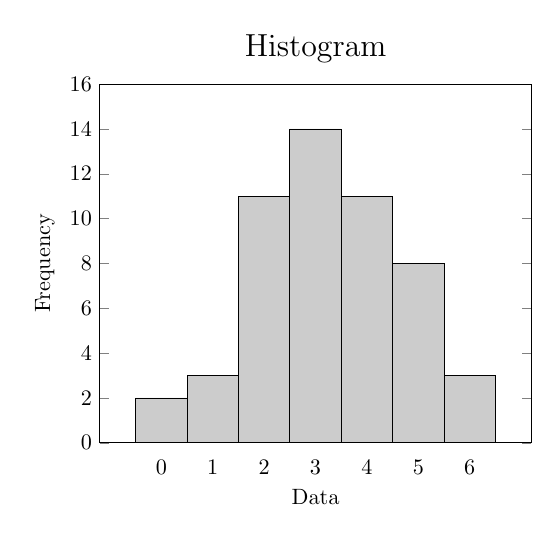
\begin{tikzpicture}[scale=0.8]
      \begin{axis}[
          title=\Large{Histogram},
          ymin=0, ymax=16,
          ytick={0, 2, ..., 16},
          xlabel=Data, ylabel=Frequency,
          ybar interval,
          grid=none,
          xtick style={draw=none},
        ]
        \addplot+[draw=black, style={fill=gray!40},mark=no] plot coordinates { (0, 2) (1, 3) (2, 11) (3, 14) (4, 11) (5, 8) (6, 3) (7, 0) };
      \end{axis}
    \end{tikzpicture}
  \end{center}

  The frequency polygon is a continuous line graph, the x-axis is the midpoint of
  each class, and the y-axis is the frequency of each class. To draw a frequency
  polygon, we plot each point, including the point before the first class and the
  point after the last class that uses $0$ as their frequency, and then connect
  the points with a continuous line.

  \begin{center}
    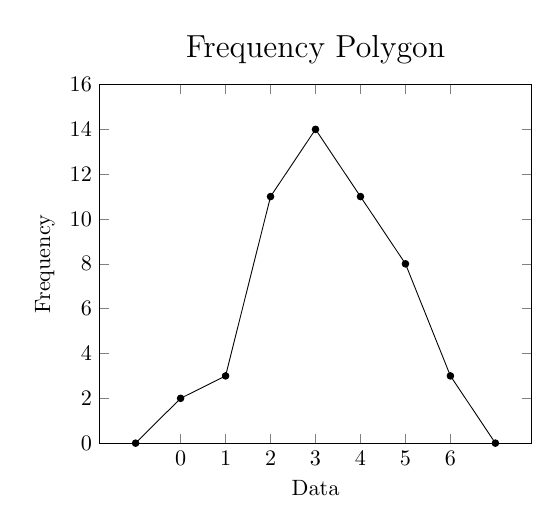
\begin{tikzpicture}[scale=0.8]
      \begin{axis}[
          title=\Large{Frequency Polygon},
          ymin=0, ymax=16,
          ytick={0, 2, ..., 16},
          xtick={0,1,...,6},
          xlabel=Data, ylabel=Frequency,
        ]
        \addplot[sharp plot, mark=*, mark size=1.5pt, mark options={solid, fill=black, draw=black}, draw=black]
        coordinates
          {(-1, 0) (0, 2) (1, 3) (2, 11) (3, 14) (4, 11) (5, 8) (6, 3) (7, 0)};
      \end{axis}
    \end{tikzpicture}
  \end{center}

  \begin{center}
    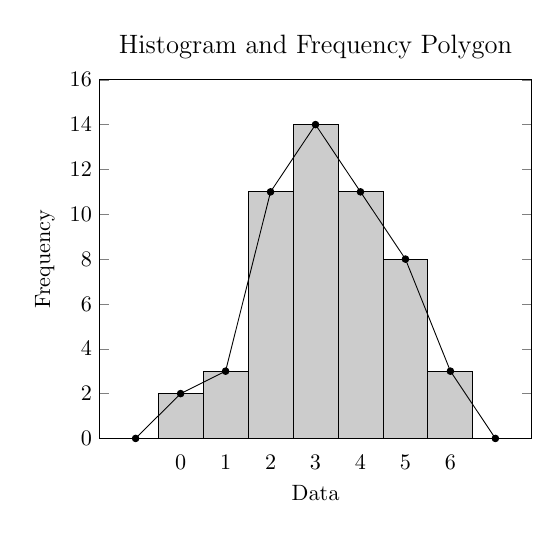
\begin{tikzpicture}[scale=0.8]
      \begin{axis}[
          title=\large{Histogram and Frequency Polygon},
          ymin=0, ymax=16,
          ytick={0, 2, ..., 16},
          xtick={0,1,...,6},
          ybar interval,
          grid=none,
          xtick style={draw=none},
          xlabel=Data, ylabel=Frequency,
        ]
        \addplot[draw=black, style={fill=gray!40},mark=no] plot coordinates { (0, 2) (1, 3) (2, 11) (3, 14) (4, 11) (5, 8) (6, 3) (7, 0) };
        \addplot[forget plot, sharp plot, mark=*, mark size=1.5pt, mark options={solid, fill=black, draw=black}, draw=black]
        coordinates
          {(-0.5, 0) (0.5, 2) (1.5, 3) (2.5, 11) (3.5, 14) (4.5, 11) (5.5, 8) (6.5, 3) (7.5, 0)};
      \end{axis}
    \end{tikzpicture}
  \end{center}

  \subsection*{Practice 1}

  There are 105 students in a senior 3 art and commerce class. In a mock exam of
  UEC, their scores for Mathematics subject are as follows:
  \begin{flalign*}
    35 & \qquad 88 \qquad 67 \qquad 32 \qquad 38 \qquad 34 \qquad 45 \\
    78 & \qquad 54 \qquad 58 \qquad 69 \qquad 21 \qquad 90 \qquad 78 \\
    74 & \qquad 43 \qquad 42 \qquad 35 \qquad 57 \qquad 34 \qquad 77 \\
    89 & \qquad 66 \qquad 74 \qquad 71 \qquad 44 \qquad 56 \qquad 48 \\
    33 & \qquad 24 \qquad 73 \qquad 63 \qquad 51 \qquad 59 \qquad 49 \\
    34 & \qquad 55 \qquad 52 \qquad 75 \qquad 72 \qquad 62 \qquad 62 \\
    44 & \qquad 48 \qquad 73 \qquad 49 \qquad 57 \qquad 67 \qquad 80 \\
    70 & \qquad 66 \qquad 54 \qquad 32 \qquad 29 \qquad 35 \qquad 37 \\
    47 & \qquad 41 \qquad 51 \qquad 36 \qquad 46 \qquad 55 \qquad 53 \\
    60 & \qquad 53 \qquad 62 \qquad 39 \qquad 35 \qquad 48 \qquad 42 \\
    71 & \qquad 63 \qquad 70 \qquad 33 \qquad 45 \qquad 42 \qquad 44 \\
    61 & \qquad 59 \qquad 67 \qquad 30 \qquad 42 \qquad 43 \qquad 89 \\
    96 & \qquad 82 \qquad 47 \qquad 63 \qquad 54 \qquad 34 \qquad 45 \\
    45 & \qquad 87 \qquad 28 \qquad 34 \qquad 29 \qquad 77 \qquad 64 \\
    64 & \qquad 50 \qquad 48 \qquad 75 \qquad 33 \qquad 56 \qquad 84
  \end{flalign*}

  \begin{enumerate}[label=(\alph*)]
    \item Find the range of the data. \sol{}
          \begin{flalign*}
            \text{Max value}         & = 96      \\
            \text{Min value}         & = 21      \\
            \therefore\ \text{Range} & = 96 - 21 \\
                                     & = 75
          \end{flalign*}

    \item Group the data into 10 classes, draw a frequency distribution table, and find
          the upper and lower boundary and midpoint of each class. \sol{}
          \begin{flalign*}
            \text{Range}             & = 75            \\
            \text{Number of classes} & = 10            \\
            \text{Class width}       & = \frac{75}{10} \\
                                     & = 7.5           \\
                                     & \approx 8
          \end{flalign*}
          \begin{center}
            \begin{tabular}{|c|c|c|c|c|}
              \hline
              \text{Score} & \text{Lower} & \text{Upper} & \text{Mid} & \text{Freq.} \\
              \hline
              21 - 28      & 20.5         & 28.5         & 24.5       & 3            \\
              29 - 36      & 28.5         & 36.5         & 32.5       & 18           \\
              37 - 44      & 36.5         & 44.5         & 40.5       & 13           \\
              45 - 52      & 44.5         & 52.5         & 48.5       & 17           \\
              53 - 60      & 52.5         & 60.5         & 56.5       & 15           \\
              61 - 68      & 60.5         & 68.5         & 64.5       & 14           \\
              69 - 76      & 68.5         & 76.5         & 72.5       & 12           \\
              77 - 84      & 76.5         & 84.5         & 80.5       & 7            \\
              85 - 92      & 84.5         & 92.5         & 88.5       & 5            \\
              93 - 100     & 92.5         & 100.5        & 96.5       & 1            \\
              \hline
            \end{tabular}
          \end{center}
    \item Draw a histogram and frequency polygon. \sol{}
          \begin{center}
            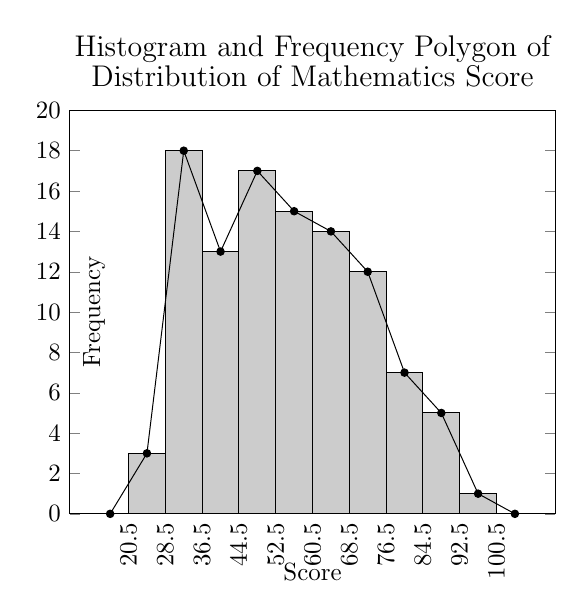
\begin{tikzpicture}[scale=0.9]
              \begin{axis}[
                  title style = {align = center},
                  title={\large{Histogram and Frequency Polygon of} \\ \large{Distribution of Mathematics Score}},
                  ymin=0, ymax=20,
                  ytick={0, 2, ..., 20},
                  xtick={20.5, 28.5, ..., 100.5},
                  grid=none,
                  xtick style={draw=none, fill=none, font=\footnotesize},
                  x tick label style = {rotate=90,anchor=east},
                  xlabel=Score, ylabel=Frequency,
                  xlabel style={at={(axis description cs:0.5, -0.1)}, anchor=north},
                  ylabel style={at={(axis description cs:0.05, 0.5)}, anchor=center},
                ]
                \addplot[ybar interval, draw=black, style={fill=gray!40},mark=no] plot coordinates { (20.5, 3) (28.5, 18) (36.5, 13) (44.5, 17) (52.5, 15) (60.5, 14) (68.5, 12) (76.5, 7) (84.5, 5) (92.5, 1) (100.5, 0) };
                \addplot[forget plot, sharp plot, mark=*, mark size=1.5pt, mark options={solid, fill=black, draw=black}, draw=black]
                coordinates
                  { (16.5, 0) (24.5, 3) (32.5, 18) (40.5, 13) (48.5, 17) (56.5, 15) (64.5, 14) (72.5, 12) (80.5, 7) (88.5, 5) (96.5, 1) (104.5, 0) };
              \end{axis}
            \end{tikzpicture}
          \end{center}
  \end{enumerate}

  \subsection*{Cumulative Frequency Distribution}

  Summing up the frequency of each class, we obtain the cumulative frequency
  distribution. Use the upper boundary of each class as the x-axis, and the
  cumulative frequency as the y-axis, we can draw the cumulative frequency
  distribution by plotting each point including the point before the first class
  that uses 0 as its frequency and connect them together. If we split the x-axis
  and the higest point of the curve into 100 equal parts, we get the percentage
  of the cumulative frequency distribution.

  \subsection*{Practice 2}

  There are 155 students in a senior 3 art and commerce class, and the frequency
  distribution table of their average marks is shown below:

  \begin{center}
    \begin{tabular}{|c|c|}
      \hline
      \text{Average Mark} & \text{Frequency} \\
      \hline
      50 - 55             & 3                \\
      55 - 60             & 8                \\
      60 - 65             & 25               \\
      65 - 70             & 38               \\
      70 - 75             & 46               \\
      75 - 80             & 19               \\
      80 - 85             & 12               \\
      85 - 90             & 4                \\
      \hline
    \end{tabular}
  \end{center}

  \begin{enumerate}[label=(\alph*)]
    \item Make a cumulative frequency distribution table and draw a cumulative frequency
          polygon.

          \sol{}
          \begin{center}
            \begin{tabular}{|c|c|c|c|}
              \hline
              \text{Avg} & \text{Freq.} & \text{Lower Than} & \text{Cumm. Freq.} \\
              \hline
              50 - 55    & 3            & 55                & 3                  \\
              55 - 60    & 8            & 60                & 11                 \\
              60 - 65    & 25           & 65                & 36                 \\
              65 - 70    & 38           & 70                & 74                 \\
              70 - 75    & 46           & 75                & 120                \\
              75 - 80    & 19           & 80                & 139                \\
              80 - 85    & 12           & 85                & 151                \\
              85 - 90    & 4            & 90                & 155                \\
              \hline
            \end{tabular}
          \end{center}

          \begin{center}
            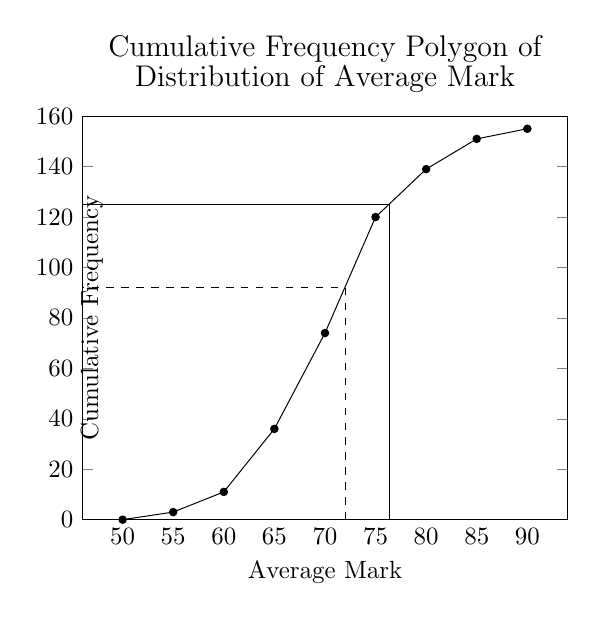
\begin{tikzpicture}[scale=0.9]
              \begin{axis}[
                  title style = {align = center},
                  title={\large{Cumulative Frequency Polygon of} \\ \large{Distribution of Average Mark}},
                  ymin=0, ymax=160,
                  ytick={0, 20, ..., 160},
                  xtick={50, 55, 60, ..., 90},
                  xtick style={draw=none, fill=none, font=\footnotesize},
                  xlabel=Average Mark, ylabel=Cumulative Frequency,
                  ylabel style={at={(axis description cs:0.02, 0.5)}, anchor=center},
                ]
                \addplot[forget plot, sharp plot, mark=*, mark size=1.5pt, mark options={solid, fill=black, draw=black}, draw=black]
                coordinates
                  { (50, 0) (55, 3) (60, 11) (65, 36) (70, 74) (75, 120) (80, 139) (85, 151) (90, 155) };
                \draw[dashed] (axis cs:72, 0) -- (axis cs:72, 92) -- (axis cs:0, 92);
                \draw (axis cs:0, 125) -- (axis cs:76.4, 125) -- (axis cs:76.4, 0);
              \end{axis}
            \end{tikzpicture}
          \end{center}

    \item If the average mark of a student is 72, find his rank in the class. \sol{}

          In the graph above, we can see that there are approximately 92 students who
          have an average mark lower than 72. Therefore, the rank of the student is $155
            - 92 = 63$.

    \item If the top $20\%$ of the class are to be awarded a certificate, find the
          minimum average mark required for the certificate. \sol{}
          \begin{flalign*}
            \text{Top $20\%$} & = 20\% \times 155 \\
                              & = 31
          \end{flalign*}
          Therefore, students with an average mark corresponding to cumulative frequency higher than 124 will be awarded a certificate.

          In the graph above, The minimum average mark required for the certificate is
          76.
  \end{enumerate}

  \subsection*{Exercise 18.2}

  \begin{enumerate}
    \item A company performed an ability test on 100 job seekers and the results are
          shown in the following table:
          \begin{center}
            \begin{tabular}{|c|c|c|c|c|c|c|}
              \hline
              \text{Score}     & 8 & 7  & 6  & 5  & 4  & 3 \\
              \hline
              \text{Frequency} & 5 & 12 & 24 & 33 & 19 & 7 \\
              \hline
            \end{tabular}
          \end{center}
          Draw a hustogram and a frequency polygon for the data above.
          \sol{}
          \begin{center}
            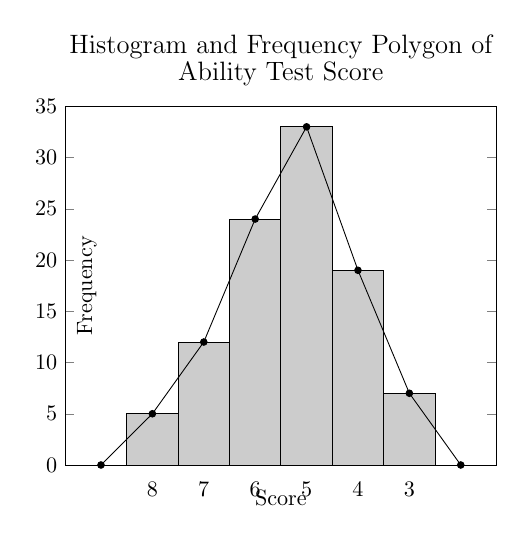
\begin{tikzpicture}[scale=0.8]
              \begin{axis}[
                  title style = {align = center},
                  title={\large{Histogram and Frequency Polygon of} \\ \large{Ability Test Score}},
                  ymin=0, ymax=35,
                  ytick={0, 5, ..., 35},
                  x dir=reverse,
                  ybar interval,
                  grid=none,
                  xtick style={draw=none},
                  xlabel=Score, ylabel=Frequency,
                  xlabel style={at={(axis description cs:0.5, -0.05)}, anchor=north},
                  ylabel style={at={(axis description cs:0.05, 0.5)}, anchor=center},
                ]
                \addplot[draw=black, style={fill=gray!40},mark=no] plot coordinates { (8, 5) (7, 12) (6, 24) (5, 33) (4, 19) (3, 7) (2, 0) };
                \addplot[forget plot, sharp plot, mark=*, mark size=1.5pt, mark options={solid, fill=black, draw=black}, draw=black]
                coordinates
                  {(8.5, 0) (7.5, 5) (6.5, 12) (5.5, 24) (4.5, 33) (3.5, 19) (2.5, 7) (1.5, 0)};
              \end{axis}
            \end{tikzpicture}
          \end{center}

    \item Take 120 ears of rice from a rice field, the length of each ear is measured (in
          $cm$) and the results are as following:
          \begin{flalign*}
            6.5 & \qquad 6.4 \qquad 6.7 \qquad 5.8 \qquad 5.9 \qquad 5.9 \\
            5.2 & \qquad 4.0 \qquad 5.4 \qquad 4.6 \qquad 5.8 \qquad 5.5 \\
            6.0 & \qquad 6.5 \qquad 5.1 \qquad 6.2 \qquad 5.4 \qquad 5.0 \\
            5.0 & \qquad 6.8 \qquad 6.0 \qquad 5.0 \qquad 5.7 \qquad 6.0 \\
            5.5 & \qquad 6.8 \qquad 6.0 \qquad 6.3 \qquad 5.5 \qquad 5.0 \\
            6.4 & \qquad 5.8 \qquad 5.9 \qquad 5.7 \qquad 6.8 \qquad 6.6 \\
            6.0 & \qquad 6.4 \qquad 5.7 \qquad 7.4 \qquad 6.0 \qquad 5.4 \\
            6.5 & \qquad 6.0 \qquad 6.8 \qquad 5.3 \qquad 6.4 \qquad 5.7 \\
            6.7 & \qquad 6.2 \qquad 5.6 \qquad 6.0 \qquad 6.7 \qquad 6.7 \\
            6.0 & \qquad 5.5 \qquad 6.2 \qquad 6.1 \qquad 5.3 \qquad 6.2 \\
            5.8 & \qquad 5.3 \qquad 7.0 \qquad 6.0 \qquad 6.0 \qquad 5.9 \\
            5.4 & \qquad 6.0 \qquad 5.2 \qquad 6.0 \qquad 6.3 \qquad 5.7 \\
            6.8 & \qquad 6.1 \qquad 4.5 \qquad 5.4 \qquad 6.3 \qquad 6.9 \\
            4.9 & \qquad 5.1 \qquad 5.6 \qquad 5.9 \qquad 6.1 \qquad 6.5 \\
            6.6 & \qquad 5.7 \qquad 5.8 \qquad 5.8 \qquad 6.2 \qquad 6.3 \\
            6.5 & \qquad 5.3 \qquad 5.9 \qquad 5.5 \qquad 5.8 \qquad 6.3 \\
            5.2 & \qquad 6.0 \qquad 7.0 \qquad 6.4 \qquad 5.8 \qquad 6.3 \\
            6.0 & \qquad 6.3 \qquad 5.6 \qquad 6.8 \qquad 6.6 \qquad 4.7 \\
            5.7 & \qquad 5.7 \qquad 5.6 \qquad 6.3 \qquad 6.0 \qquad 5.8 \\
            6.3 & \qquad 7.5 \qquad 6.2 \qquad 6.4 \qquad 7.0 \qquad 6.5
          \end{flalign*}

          \begin{enumerate}
            \item Find the range of the dataset. \sol{}
                  \begin{flalign*}
                    \text{Min value}         & = 4.0       \\
                    \text{Max value}         & = 7.5       \\
                    \therefore\ \text{Range} & = 7.5 - 4.0 \\
                                             & = 3.5
                  \end{flalign*}
            \item Group the data into 12 classes, make a frequency distribution table, find the
                  upper and lower boundaries and midpoint of each class, and calculate the
                  cumulative frequency. \sol{}
                  \begin{flalign*}
                    \text{Range}                   & = 3.5            \\
                    \text{Number of classes}       & = 12             \\
                    \therefore\ \text{Class width} & = \frac{3.5}{12} \\
                                                   & = \frac{3.5}{12} \\
                                                   & \approx 0.3
                  \end{flalign*}
                  \begin{center}
                    \begin{tabular}{|c|c|c|c|c|}
                      \hline
                      Weight    & Lower & Upper & Mid  & Freq. \\
                      \hline
                      4.0 - 4.2 & 3.95  & 4.25  & 4.10 & 1     \\
                      4.3 - 4.5 & 4.25  & 4.55  & 4.40 & 1     \\
                      4.6 - 4.8 & 4.55  & 4.85  & 4.70 & 2     \\
                      4.9 - 5.1 & 4.85  & 5.15  & 5.00 & 7     \\
                      5.2 - 5.4 & 5.15  & 5.45  & 5.30 & 12    \\
                      5.5 - 5.7 & 5.45  & 5.75  & 5.60 & 17    \\
                      5.8 - 6.0 & 5.75  & 6.05  & 5.90 & 31    \\
                      6.1 - 6.3 & 6.05  & 6.35  & 6.20 & 18    \\
                      6.4 - 6.6 & 6.35  & 6.65  & 6.50 & 15    \\
                      6.7 - 6.9 & 6.65  & 6.95  & 6.80 & 11    \\
                      7.0 - 7.2 & 6.95  & 7.25  & 7.10 & 3     \\
                      7.3 - 7.5 & 7.25  & 7.55  & 7.40 & 2     \\
                      \hline
                    \end{tabular}
                  \end{center}
                  \begin{center}
                    \begin{tabular}{|c|c|c|c|}
                      \hline
                      Weight    & Freq. & Lower Than & Cumm. Freq. \\
                      \hline
                      4.0 - 4.3 & 1     & 4.3        & 1           \\
                      4.3 - 4.6 & 1     & 4.6        & 2           \\
                      4.6 - 4.9 & 2     & 4.9        & 4           \\
                      4.9 - 5.2 & 7     & 5.2        & 11          \\
                      5.2 - 5.5 & 12    & 5.5        & 23          \\
                      5.5 - 5.8 & 17    & 5.8        & 40          \\
                      5.8 - 6.1 & 31    & 6.1        & 71          \\
                      6.1 - 6.4 & 18    & 6.4        & 89          \\
                      6.4 - 6.7 & 15    & 6.7        & 104         \\
                      6.7 - 7.0 & 11    & 7.0        & 115         \\
                      7.0 - 7.3 & 3     & 7.3        & 118         \\
                      7.3 - 7.6 & 2     & 7.6        & 120         \\
                      \hline
                    \end{tabular}
                  \end{center}

            \item Draw a frequency polygon. \sol{}
                  \begin{center}
                    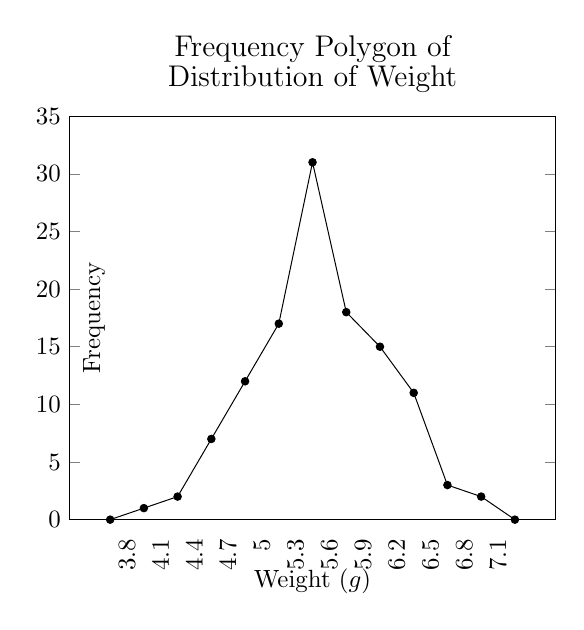
\begin{tikzpicture}[scale=0.9]
                      \begin{axis}[
                          title style = {align = center},
                          title={\large{Frequency Polygon of} \\ \large{Distribution of Weight}},
                          ymin=0, ymax=35,
                          ytick={0, 5, ..., 35},
                          ybar interval,
                          grid=none,
                          xtick style={draw=none, fill=none, font=\footnotesize},
                          x tick label style = {rotate=90,anchor=east},
                          xlabel=Weight ($g$), ylabel=Frequency,
                          xlabel style={at={(axis description cs:0.5, -0.1)}, anchor=north},
                          ylabel style={at={(axis description cs:0.05, 0.5)}, anchor=center},
                        ]
                        \addplot[forget plot, sharp plot, mark=*, mark size=1.5pt, mark options={solid, fill=black, draw=black}, draw=black]
                        coordinates
                          { (3.8, 0) (4.1, 1) (4.4, 2) (4.7, 7) (5.0, 12) (5.3, 17) (5.6, 31) (5.9, 18) (6.2, 15) (6.5, 11) (6.8, 3) (7.1, 2) (7.4, 0) };
                      \end{axis}
                    \end{tikzpicture}
                  \end{center}

            \item Draw a cumulative frequency polygon. \sol{}
                  \begin{center}
                    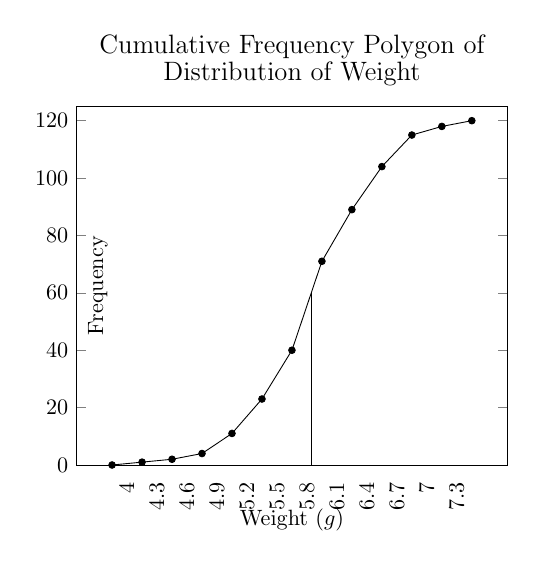
\begin{tikzpicture}[scale=0.8]
                      \begin{axis}[
                          title style = {align = center},
                          title={\large{Cumulative Frequency Polygon of} \\ \large{Distribution of Weight}},
                          ymin=0, ymax=125,
                          ytick={0, 20, ..., 120},
                          ybar interval,
                          grid=none,
                          xtick style={draw=none, fill=none, font=\footnotesize},
                          x tick label style = {rotate=90,anchor=east},
                          xlabel=Weight ($g$), ylabel=Frequency,
                          xlabel style={at={(axis description cs:0.5, -0.1)}, anchor=north},
                          ylabel style={at={(axis description cs:0.05, 0.5)}, anchor=center},
                        ]
                        \addplot[forget plot, sharp plot, mark=*, mark size=1.5pt, mark options={solid, fill=black, draw=black}, draw=black]
                        coordinates
                          { (4.0, 0) (4.3, 1) (4.6, 2) (4.9, 4) (5.2, 11) (5.5, 23) (5.8, 40) (6.1, 71) (6.4, 89) (6.7, 104) (7.0, 115) (7.3, 118) (7.6, 120) };
                        \draw (axis cs: 6, 0) -- (axis cs: 6, 60);
                      \end{axis}
                    \end{tikzpicture}
                  \end{center}
            \item Find the percentage of the ears of rice whose length is greater than $6cm$.
          \end{enumerate}

    \item The table below shows the weight distribution of 90 babies (in $kg$):
          \begin{center}
            \begin{tabular}{|c|c|}
              \hline
              Weight    & Frequency \\
              \hline
              1.5 - 2.0 & 2         \\
              2.0 - 2.5 & 4         \\
              2.5 - 3.0 & 13        \\
              3.0 - 3.5 & 32        \\
              3.5 - 4.0 & 28        \\
              4.0 - 4.5 & 10        \\
              4.5 - 5.0 & 1         \\
              \hline
            \end{tabular}
          \end{center}
          \begin{enumerate}
            \item Make a cumulative frequency table.
            \item Draw a cumulative frequency polygon.
            \item Find the percentage of babies whose weight is greater than $3.8kg$.
          \end{enumerate}

    \item The table below shows the average score distribution of 50 students in a class:
          \begin{center}
            \begin{tabular}{|c|c|}
              \hline
              Average Score & Frequency \\
              \hline
              50.0 - 59.9   & 4         \\
              60.0 - 69.9   & 9         \\
              70.0 - 79.9   & 23        \\
              80.0 - 89.9   & 12        \\
              90.0 - 99.9   & 2         \\
              \hline
            \end{tabular}
          \end{center}
          \begin{enumerate}
            \item Make a cumulative frequency table and draw a cumulative frequency polygon.
            \item A student get an average score of $74$, find his rank in the class.
            \item Find the average score of the student who is ranked $20$.
            \item Find the percentage of students whose average score is greater than $85$.
          \end{enumerate}

    \item The table below shows the score distribution of 1200 students in UEC accounting
          exam:
          \begin{center}
            \begin{tabular}{|c|c|}
              \hline
              Score   & Number of Students \\
              \hline
              10 - 19 & 20                 \\
              20 - 29 & 60                 \\
              30 - 39 & 95                 \\
              40 - 49 & 130                \\
              50 - 59 & 340                \\
              60 - 69 & 310                \\
              70 - 79 & 135                \\
              80 - 89 & 80                 \\
              90 - 99 & 30                 \\
              \hline
            \end{tabular}
          \end{center}
          Examinees are categorised into 4 groups based on their score: \textit{Excellent}, \textit{Good}, \textit{Pass}, and \textit{Fail}.
          \begin{enumerate}
            \item Make a cumulative frequency table and draw a cumulative frequency polygon.
            \item If the passing score is $38$, find the percentage of students who pass the
                  exam.
            \item Assume that the minimum score to be categorised as \textit{Excellent} and
                  \textit{Good} is $75$ and $55$ respectively, find the percentage of students
                  who are categorised as \textit{Excellent} and \textit{Good} respectively.
            \item Find the passing mark if the percentage of students who pass the exam is
                  $90\%$.
            \item Find the minimum mark of a student who is categorised as \textit{Excellent} if
                  the percentage of students who are categorised as \textit{Excellent} is $15\%$.
          \end{enumerate}

  \end{enumerate}

  \section{Central Tendency}

  \section{Measures of Dispersion}

  \section{Coefficient of Variation}

  \section{Correlation and Correlation Coefficient}

  \section{Statistical Index}

  \chapter{Permutations and Combinations}

  \section{Addition and Multiplication Principles}

  \section{Permutations and Permutation Formula}

  \section{Circular Permutations}

  \section{Full Permutations of Inexactly Distinct Elements}

  \section{Permutations with Repetition}

  \section{Combinations and Combination Formula}

  \chapter{Bionomial Theorem}

  \section{Bionomial Theorem when $n$ is a Natural Number}

  \section{General Form of Bionomial Expansion}

  \chapter{Probability}

  \section{Sample Space and Events}

  \section{Definition of Probability}

  \section{Addition Rule}

  \section{Multiplication Rule}

  \section{Mathematical Expectation}

  \section{Normal Distribution}
\end{multicols}

\end{document}